\documentclass[12pt]{article}
\usepackage[margin=2.5cm]{geometry}
\usepackage{enumerate}
\usepackage{amsfonts}
\usepackage{amsmath}
\usepackage{fancyhdr}
\usepackage{amsmath}
\usepackage{amssymb}
\usepackage{amsthm}
\usepackage{mdframed}
\usepackage{graphicx}
\usepackage{subcaption}
\usepackage{adjustbox}
\usepackage{listings}
\usepackage{xcolor}
\usepackage{courier}
\usepackage[utf]{kotex}
\usepackage{hyperref}
\usepackage{soul}
\usepackage{cancel}


\definecolor{codegreen}{rgb}{0,0.6,0}
\definecolor{codegray}{rgb}{0.5,0.5,0.5}
\definecolor{codepurple}{rgb}{0.58,0,0.82}
\definecolor{backcolour}{rgb}{0.95,0.95,0.92}

\lstdefinestyle{mystyle}{
    backgroundcolor=\color{backcolour},
    commentstyle=\color{codegreen},
    keywordstyle=\color{magenta},
    numberstyle=\tiny\color{codegray},
    stringstyle=\color{codepurple},
    basicstyle=\ttfamily\footnotesize,
    breakatwhitespace=false,
    breaklines=true,
    captionpos=b,
    keepspaces=true,
    numbers=left,
    numbersep=5pt,
    showspaces=false,
    showstringspaces=false,
    showtabs=false,
    tabsize=1
}

\lstset{style=mystyle}

\pagestyle{fancy}
\renewcommand{\headrulewidth}{0.4pt}
\lhead{CSC 369}
\rhead{Notes}

\begin{document}
\title{CSC 369 Notes}

\begin{enumerate}[1.]
    \item \textbf{Secondary Storage Devices}

    \begin{itemize}
        \item
    \end{itemize}
    \item \textbf{Disk Components}

    \begin{center}
    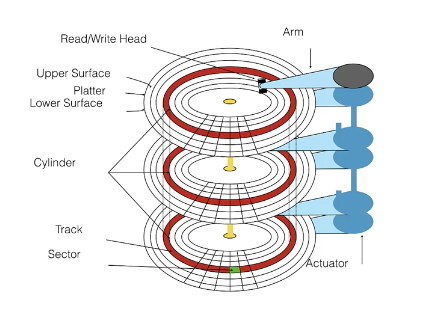
\includegraphics[width=0.8\linewidth]{images/notes_1.png}
    \end{center}

    \begin{itemize}
        \item Parts
        \begin{itemize}
            \item \textbf{Platter:}
            \begin{itemize}
                \item Data can be stored in both upper and lower parts of the platter
            \end{itemize}
            \item \textbf{Cyliner:}
            \begin{itemize}
                \item Is a set of tracks that can be read without moving the arm
            \end{itemize}
            \item \textbf{Sector:}
            \begin{itemize}
                \item Size of disk block is multiple of sectors
            \end{itemize}
        \end{itemize}
        \item Disk arm touching surface $\to$ disk suface crash
    \end{itemize}
    \item \textbf{Disk Performance}
    \begin{itemize}
        \item \textbf{Seek:}
        \begin{itemize}
            \item Is the time it takes to move the disk arm to correct cylinder
        \end{itemize}
        \item \textbf{Rotation:}
        \item \textbf{Transfer:}
    \end{itemize}
    \item \textbf{Track Skew}
    \begin{itemize}
        \item compensates the time of disk arm moving from one track to next
        \item Is to reduce rotational latency
    \end{itemize}
\end{enumerate}


\end{document}
